% !TEX root = ../Dokumentation.tex
\section{Realisierung}

\subsection{RaspberryPi}

Folgende Installation \& Grundkonfigurationen müssen zu Beginn am RaspberryPi vorgenommen werden.

\subsubsection{Software}
Die 32GB grosse SD-Karte welche man für das Raspberry benötigt, wird zu Beginn formatiert um danach eine saubere Installation des Betriebssystems durchzuführen. Als OS wird die Version 2017-04-10 raspbian-jessie verwedent, dieses Betriebssystem wird von diversen Webseiten und Anleitungen empfohlen. Es hat eine graphische Oberfläche und bietet bereits vorinstallierte Programme.


\subsubsection{Konfiguration}
Nach der Installation der Software kann das Raspberry mit Maus und Tastatur an einen Monitor angeschlossen werden. Sobald das Raspberry mit Strom versorgt wird, startet der Boot-Vorgang.
Nun müssen alle wichtigen Grundkonfigurationen wie folgt vorgenommen werden.

Tastatur: Deutsch(Schweiz)
Username: TemperatureSensorPi\\
Passwort: temperatur2017\\
Inteface SPI: enable\\
Netzwerk: <tbd>

\subsubsection{Webserver}
Auf dem Raspberry wird zusätzlich ein Webserver bereitgestellt, damit die die Temperaturausgabe direkt im lokalen Netz betrachtet werden kann. Als Webserver wurde Apache2 installiert.


\subsection{Softwaredesing}

Im untenstehenden Klassendiagramm sind alle erstellten Klassen ersichtlich.
Die Klasse SensorWatchDog ist dafür zuständig um die angeschlossenen Sensoren zu prüfen, wird ein neuer Sensor angeschlossen, so wird dieser mit der Methode addSensor in der Klasse Controller hinzugefüg. Die Klasse SensorHandler überprüft und berechnet nun laufend die Temperaturwerte. Der Wert des Sensors wird schlussendlich mittels XMLWriter in das File sensordata.xml geschrieben. Dieses File wird für die Ausgabe auf der Webseite benötigt.
Ebenfalls gibt es eine Logger-Klasse welche alle Meldungen mit einem Zeitstempel in ein Logfile schreibt. So kann genau überprüft werden, wann ein Sensor angeschlossen oder entfernt wurde aber auch ob zum richtigen Zeitpunkt ein Mail versendet wurde. 

\begin{figure}[H]%Position festigen
\centering
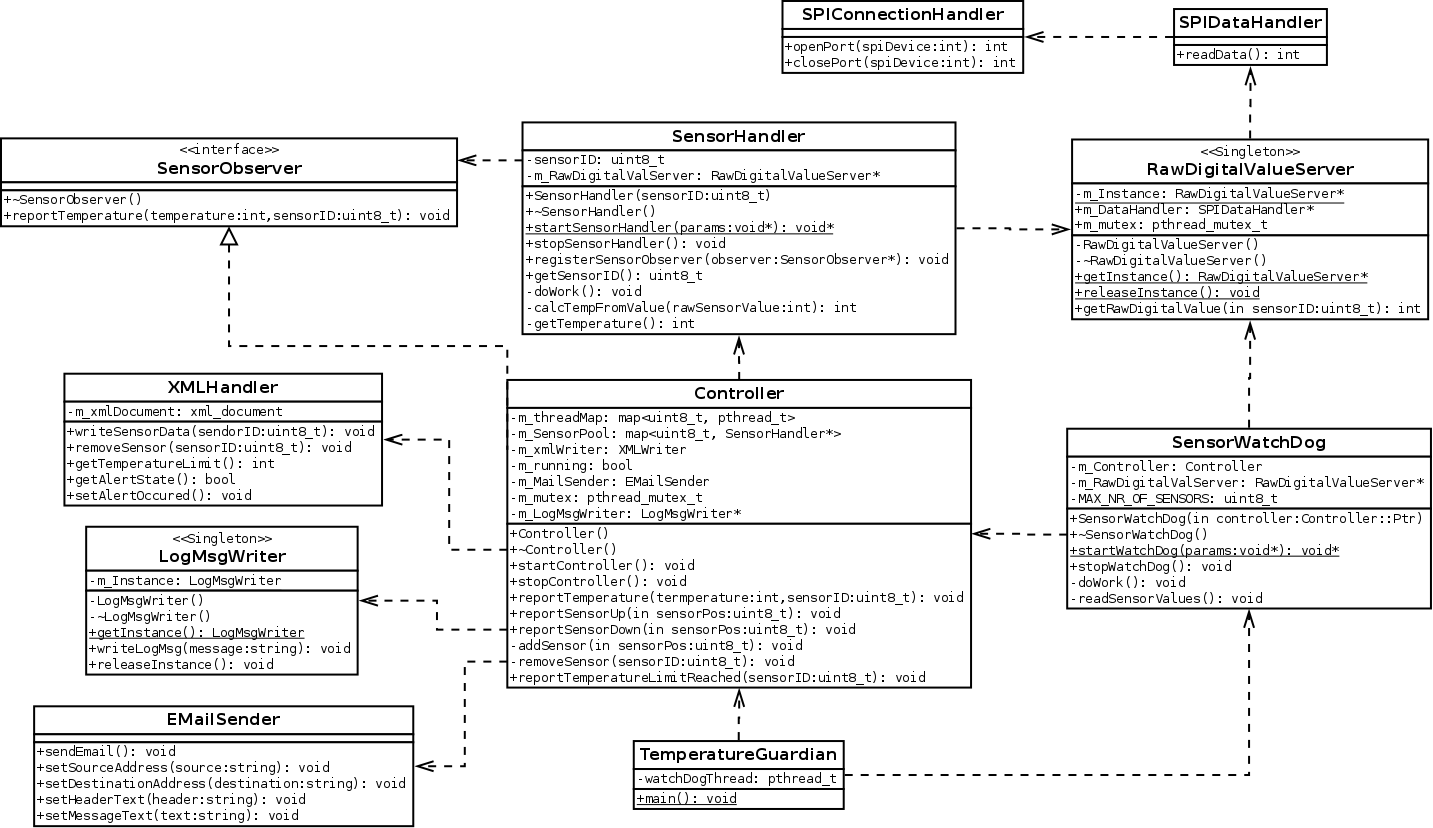
\includegraphics[width=1\textwidth]{Images/Klassendiagramm.png}
\caption{Klassendiagramm Software}
\label{fig:classdia}
\end{figure}
\subsection{Verwendete Hardware}

\begin{figure}[H]%Position festigen
\centering
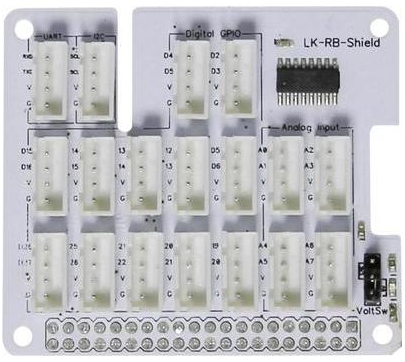
\includegraphics[width=0.25\textwidth]{Images/Basisplatine.jpg}
\caption{Basisplatine zum Raspberry Pi (Quelle www.Conrad.ch)}
\label{fig:plate}
\end{figure}

\begin{figure}[H]%Position festigen
\centering
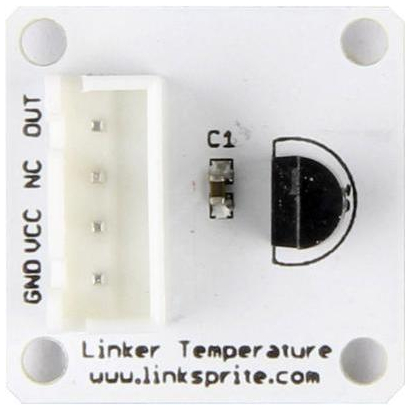
\includegraphics[width=0.25\textwidth]{Images/Sensorplatine.jpg}
\caption{Sensorplatine mit Temperaturfühler (Quelle www.Conrad.ch)}
\label{fig:sensor}
\end{figure}

\begin{figure}[H]%Position festigen
\centering
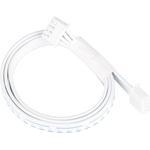
\includegraphics[width=0.25\textwidth]{Images/Verbindungskabel.jpg}
\caption{Verbindungskabel (Quelle www.Conrad.ch)}
\label{fig:cable}
\end{figure}

\subsection{Webdarstellung}
Die Umsetzung der Webseite wurde hauptsächlich mit JavaScript gemacht.
Für die Anzeige der Temperatur wurde das JavaScript Plugin JustGage verwendet. Diese visuelle Darstellung ermöglicht es, auf 1 Blick zu erkenn, ob die aktuellen Werte zu hoch oder allenfalls zu niedrig sind.\\

Die Werte werden von der Software als XML-File geliefert, in welchem die Temperaturwerte pro Sensor gespeichert sind. Die Webseite wurde so konzipiert, dass dieses XML-File in einem regelmässigen Zyklus gelesen und entsprechend auf der Seite ausgegeben wird. Dieser Punkt gehört mitunter zu einer der wichtigsten, denn die korrekte Anzeige der Temperaturwerte ist notwendig um die Kontrolle zu jederzeit zu gewährleisten. Diese Anforderung kann setInterval(function, 1000) umgesetzt werden. Mit dieser Funktion werden die Temperaturwerte jede Sekunde oder nach Belieben neu vom XML-File gelesen.
Zusätzlich bringt JustGage die Funktion mit sich, welche es ermöglicht über refresh(val) dem Sensor die neuen Werte zu übergeben.\\


\textbf{Beispielcode der Webseite}

\begin{lstlisting}{}
//Erstellen eines Sensors
var s1 = new JustGage({
	id: "s1",
	alue: 0,
    min: 0,
    max: 75,
    title: "Sensor 1",
    hideMinMax: true
});

//Auslesen der Temperaturwerte
function readXMLNode(xml) {
	var xmlDoc = xml.responseXML;
	for (var i = 0, len = valueArray.length; i < len; i++) {
	valueArray[i] = xmlDoc.getElementsByTagName("SensorValues")[0].getElementsByTagName("Sensor")[i].getAttribute("value");
	}
};

//Zyklische Uebergabe der Temperaturwerte an den Sensor
setInterval(function () {
	loadXmlFile();
	s1.refresh(valueArray[0]);
}, 1000);
\end{lstlisting}

\begin{figure}[H]%Position festigen
\centering
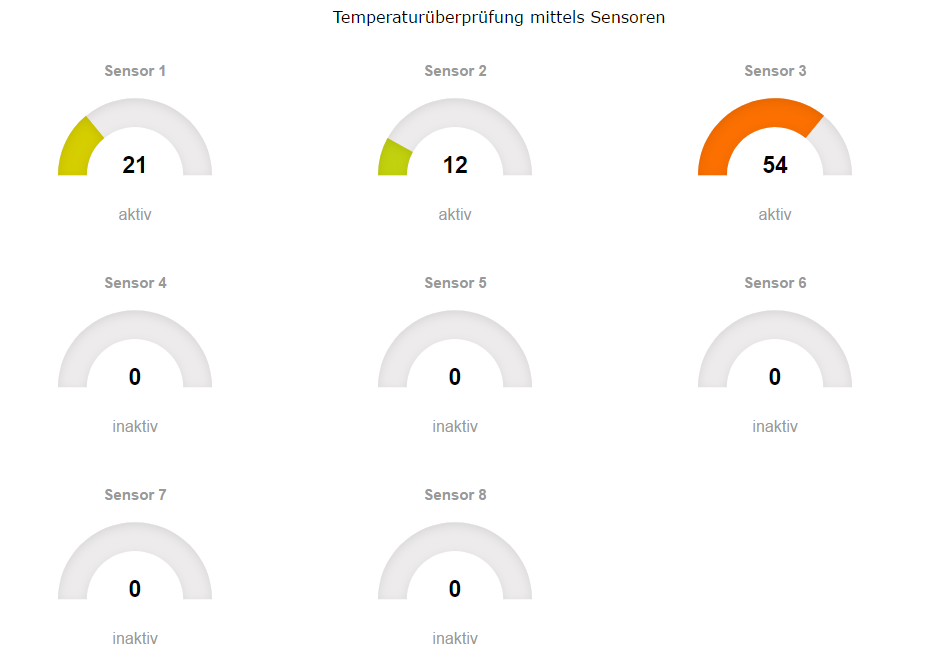
\includegraphics[width=0.5\textwidth]{Images/Webseite.png}
\caption{Ausgabe der Webseite}
\label{fig:classdia}
\end{figure}

\section{Versuchsdurchführung}